\documentclass[conference]{IEEEtran}

\usepackage{cite}
\usepackage{pslatex} % -- times instead of computer modern, especially for the plain article class
\usepackage[colorlinks=false,bookmarks=false]{hyperref}
\usepackage{booktabs}
\usepackage{graphicx}
\usepackage{xcolor}
\usepackage{multirow}
\usepackage{comment}

\usepackage{listings}
\lstset{
	columns=fullflexible,
	%        basicstyle=\ttfamily\footnotesize,
	basicstyle=\ttfamily\small,      
	%columns=fullflexible, keepspaces=true,
	numbers=left,    
	numberblanklines=false,
	captionpos=b,
	%	breaklines=true,
	escapeinside={@}{@},
	numbersep=5pt,
	language=C,
	tabsize=2,
	breakatwhitespace=true,
	breaklines=true,
	deletekeywords={for},
	%        keywordstyle=\ttfamily
	numbersep=5pt,
	xleftmargin=.10in,
	%xrightmargin=.25in
}
%\usepackage{flushend} % even out the last page, but use only at the end when there is a bibliography

\newcommand{\code}[1]{{\small{\texttt{#1}}}}

% fatter TT font
\renewcommand*\ttdefault{txtt}
% another TT, suggested by Alex
% \usepackage{inconsolata}
% \usepackage[T1]{fontenc} % needed as well?

\usepackage{listings}

%\newcommand{\todo}[1]{{\emph{TODO: #1}}}
\newcommand{\todo}[1]{{\color{olive} TODO: #1}}
\newcommand{\martin}[1]{{\color{blue} Martin: #1}}
\newcommand{\andrew}[1]{{\color{red} Andrew: #1}}
\newcommand{\tjark}[1]{{\color{orange} Tjark: #1}}
\newcommand{\rewrite}[1]{{\color{red} rewrite: #1}}

% uncomment following for final submission
%\renewcommand{\todo}[1]{}
%\renewcommand{\martin}[1]{}


%%Uncomment the following when you want to add copyright notice and not use any space	 (IEEE only)
%\usepackage[absolute]{textpos}
%% Set unit to be pagewidth and height, and increase inner margin of box
%\setlength{\TPHorizModule}{\paperwidth}\setlength{\TPVertModule}{\paperheight}
%\TPMargin{5pt}
%% Define \copyrightstatement command for easier use
%\newcommand{\copyrightstatement}{
%	\begin{textblock}{0.85}(0.072,0.93)    % Tweak here: {box width}(leftposition, rightposition)
%		\noindent
%		\normalsize
%		???-?-?-???-?/??/\$31.00~\copyright20?? IEEE % Put here your copyright
%	\end{textblock}
%}

\begin{document}


%\title{Towards Verification of Digital Circuits with\\
%SystemVerilog/UVM and Chisel/Scala}

\title{Functional Coverage-Driven Fuzzing\\ for Chisel Designs}

\author{


\IEEEauthorblockN{Andrew Dobis, Tjark Petersen, Martin Schoeberl}
\IEEEauthorblockA{\textit{Department of Applied Mathematics and Computer Science} \\
\textit{Technical University of Denmark}\\
Lyngby, Denmark \\
adobis@student.ethz.ch, s186083@student.dtu.dk, masca@dtu.dk}
}


\maketitle \thispagestyle{empty}

\begin{abstract}

Verification of digital systems must verified in ever tighter time constraints due to the rise of domain-specific hardware accelerators.
To combat this, we can learn from agile techniques used in software engineering and bringing them to the hardware design.
In this mindset, Chisel, a hardware construction language embedded in Scala, was developed as a tool to accelerate the implementation of digital designs.
Following this path, we developed a high-level verification library named ChiselVerify, bringing tools such as functional coverage to the Chisel ecosystem.
Using this tool, we propose a functional coverage-driven mutation-based fuzzer for Chisel designs.
Initial experiments are done on the Leros accumulator ALU.

\end{abstract}

\begin{IEEEkeywords}
digital design, verification, fuzzing, coverage
\end{IEEEkeywords}
\section{Introduction}
\label{sec:intro}

In recent years, we have seen an increase in the demands for high performance computing systems.  
This comes with an increase in the need for domain-specific hardware accelerators.  
Designing these is time-consuming and error prone, which is why researchers have been focusing on increasing the efficiency of hardware design and verification tools to fight this added time constraint.
This has lead to the introduction of verifications methods, such as constrained random verification and functional coverage~\cite{verify:chisel:2020, dobis2021opensource}, into high level hardware construction languages, like the Scala-embedded language Chisel~\cite{chisel:dac2012, chisel:book} .
These tools, inspired by the more hardware-centric approach given in SystemVerilog and UVM, enable basic verification where the user has to handle the writing of all tests by hand.
To improve the efficiency of these tools, we propose a form of dynamic verification, based on coverage-driven mutation-based fuzzing techniques found in the software world.
This allows for optimal fuzzing for digital designs using functional coverage as a metric to drive the fuzzing.

This paper describes a research project that aims to develop a functional coverage-driven mutation-based fuzzing tool to test digital circuits.
Furthermore, we plan to build on this tool to generate constrained random programs so that fuzzing can be used to test processors.

This paper is organized in six sections: % The following section presents related work.
Section~\ref{sec:related}  presents related work.
Section~\ref{sec:tools} describes the open-source tools that we use in our project.
Section~\ref{sec:fuzz} presents our open-source fuzzing library, which is part of ChiselVerify.
Section~\ref{sec:eval} evaluates our approach with a small design example written in Chisel.
Section~\ref{sec:conclusion} concludes.


\section{Related Work}
\label{sec:related}

The Universal Verification Methodology (UVM) is a methodology for testing and verifying of digital circuits.
UVM is implemented as a SystemVerilog library and utilizes the fact that SystemVerilog uses object-oriented programming when designing test-benches.
Using object-oriented patterns such as inheritance and polymorphism, the verification engineer can design generic components that can be extended and modified to provide application-specific functionality.
As of 2017, UVM has been standardized as IEEE 1800.2~\cite{IEEE:18002}.
UVM is a first step towards truly standardized test-benches.

At the time of writing, little published work was done in the realm of fuzzing for digital circuits.
One project, named RFuzz~\cite{rfuzz2018} and lead by researchers at UC Berkeley, focuses on ``coverage-guided fuzz mutational testing''. This method relies on FPGA-accelerated simulation and new solutions allowing for quick and deterministic memory resetting, to efficiently use fuzzing on digital circuits. The coverage metrics used in this solution are automated and based on branch coverage. RFuzz is currently no longer in development (last commit is from July 2020). RFuzz differs from what we present in this paper in two ways. First, RFuzz uses a simple coverage metric that is independent of the device under test (DUT), while we guide our fuzzing using functional coverage, which inherently contains information about the DUT. Functional coverage is obtained using tools from ChiselVerify~\cite{verify:chisel:2020, dobis2021opensource}.
Another difference is in the randomized program generation, while RFuzz only generates random bit streams, our goal is to focus as well on the generation of coherent random generated programs to test a processor.

American fuzzy loop (AFL)~\cite{afl:repo} is a mutation-based fuzzer for software developed by researchers at Google. 
AFL uses a form of branch coverage, known as edge coverage, as a driving metric.
RFuzz, as well as our own solution, is based on AFL. 
The key difference is that AFL is a fuzzer for software, while the two other fuzzers are for digital circuits.
This impacts the way a test is defined, interpreted and mutated~\cite{rfuzz2018}.

As for random program generation, the open-source RISC-V DV framework \cite{riscvdv}, built using python and SystemVerilog, is a notable existing solution. 
However, an implementation in Scala will have the advantage of keeping all internal communications in the same language. 
Our implementation will also not limit itself to one ISA but will provide a general infrastructure for RISC architectures and ISA definitions will be kept as libraries.

As far as we know, our solution, which is part of the verification library ChiselVerify, is the only mutation-based fuzzer for digital circuits that uses functional coverage to drive the test generation.

\section{Open-Source Tools}
\label{sec:tools}

Our work is based on the methods and heuristics used in AFL, which we reimplement in Scala in order to use it along with other Chisel verification libraries like ChiselTest~\cite{chisel:tester2} and ChiselVerify.
%To understand this tool, we must first describe how mutation-based fuzzing works.

\subsection{Mutation-based Fuzzing}
Mutation-based fuzzing is a form of blackbox fuzzing, i.e., fuzzing where the fuzzing engine does not know about the program or device it is testing.
\begin{figure}
  \centering
    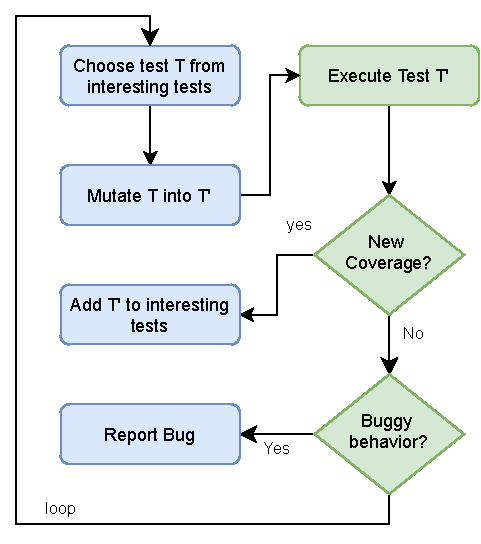
\includegraphics[width=0.9\linewidth]{mutation-fuzzing.pdf}
    \caption{Mutation-based fuzzing feedback loop. First start with a test, i.e.\, with a set of inputs, then mutate the test, execute it and evaluate how it effected the coverage. If the coverage changed, then the test is interesting else it is not.}
\label{fig:mut-fuzz}
\end{figure}

Figure~\ref{fig:mut-fuzz} shows that, in mutation-based fuzzing, we start by defining well-formed inputs, a.k.a.\ seeds, and a coverage metric. 
We then mutate the seeds based on coverage feedback from a previous test in order to obtain new coverage results. 
The fuzzing stops once a target coverage percentage is reached.

We can then define a fuzzer with 3 elements:
\begin{itemize}
\item \textbf{Fuzz server}, which interfaces with the program under test and resets it after each test.
\item \textbf{Instrumentation pass}, which is where the coverage-related modifications are made to the program under test.
\item \textbf{Fuzz engine}, which handles test mutation and coverage-feedback analysis.
\end{itemize}

\subsection{Chisel}
Our project focuses on digital circuits designed in Chisel.
Chisel is a hardware construction language embedded in Scala~\cite{chisel:dac2012} that generates Verilog as a final output.
Chisel also generates code in an intermediate representation named \texttt{FIRRTL}\footnote{\url{https://github.com/freechipsproject/firrtl}}.(Flexible Intermediate Representation for RTL).
Chisel allows the user to describe digital circuits in a high-level manner, using functional tools and libraries from Scala in order to minimize the amount of code needed to describe a circuit.
Since Chisel is a pure hardware \emph{construction} language, all valid Chisel code maps to synthesizable hardware.
Chisel also enables the verification engineer to use the full power of Scala and Java in a Chisel test-bench, thus making the verification more efficient.

\subsection{ChiselTest}
 
There a several ways to test a Chisel design, where the most common is to write test-benches for the emitted Verilog code.
This may be done with standard Verilog test-benches or writing more complex ones using SystemVerilog with UVM.
 
ChiselTest~\cite{chisel:tester2}, a non-synthesizable testing framework for Chisel, offers another solution by allowing one to directly test the Chisel code in a usable and simple way.
ChiselTest works as a Scala library that allows the user to interface directly with the simulator with operations like \texttt{peek} (view the value of a wire), \texttt{poke} (write a value to a wire) and \texttt{step} (increment the clock).
In order to write concurrent test-benches, the library also offers a \texttt{fork} method.

ChiselTest tries to enable best practices from software engineering by having lightweight syntax, allowing one to easily write small targeted unit tests.
Our project uses ChiselTest as a backend in order to access the simulator throughout the fuzzing cycle.

\subsection{ChiselVerify}

The presented fuzzer is part of the ChiselVerify project~\cite{verify:chisel:2020, dobis2021opensource}, available
at \url{https://github.com/chiselverify}.

ChiselVerify's functional coverage tool is used as the driving metric of our fuzzer.
Functional coverage is a hardware-oriented coverage metric that helps verify how thoroughly certain features of a given specification have been tested.
These features are defined in what's called a \textit{verification plan}~\cite{spear2008systemverilog}, which is defined using a set of \texttt{cover} constructs. 
A \texttt{cover} construct is associated to one or many DUT ports, and contains \texttt{bins} defining a range or a condition to sample over.
A \texttt{hit} is considered when a value sampled for the port is either contained in the bin's range or validates its condition.

\subsection{Simulators}

Chisel designs can be simulated by simulating the generated Verilog or FIRRTL code.
Verilog can be used by any Verilog simulator.
Most of them, however, are proprietary and thus need expensive licenses in order to be used. 
The main open-source option is \texttt{verilator}~\cite{verilator}, which has a high compilation cost but has a good per-cycle efficiency.

The second option is to use a FIRRTL simulator, the main one being Treadle.\footnote{\url{https://github.com/freechipsproject/treadle}}
Treadle operates on FIRRTL and thus allows one to avoid generating Verilog code, which can vastly reduce the setup time for tests and efficiently run suites of many short tests.
ChiselTest and our solution use Treadle as a simulator. 

\section{Fuzzing with Chisel}
\label{sec:fuzz}
The main goal of this project is to enable the fuzzing of digital circuits implemented in Chisel, while using functional coverage as a driving metric.
As a first attempt, we used AFL's mutation engine using the Java Native Interface (JNI).
In order to reduce compilation time, we chose to reimplement a subset of AFL's mutation techniques using Scala.
We will now present the fuzzer's current structure.

The fuzzer works in five main phases:  
\begin{itemize}
\item Interpret user-defined input files as bit-streams and load them into a queue.
\item Select the next file from said queue.
\item Mutate the file, using multiple passes of first deterministic then non-deterministic mutation techniques.  
\item Run the test and retrieve coverage results. 
\item Compare the results to the previous ones to determine if the new test was interesting or not. Add the test to the corpus of interesting tests if needed and repeat. 
\end{itemize}  

Initial inputs are defined by the user and will be the base seeds of the test corpus.
This is done by defining a set of binary seed files that each contain a sequence of inputs for the DUT.

We define the input size as the sum of the bit length of all input signals of the DUT.
\begin{lstlisting}[captionpos=b,caption={Basic DUT with two 32 bit inputs, one 64 input, as well as a 32 bit output.},label={lst:dutexample},language=scala]
class DUT extends Module {
    val io = IO(new Bundle {
        val inA = Input(UInt(32.W))
        val inB = Input(UInt(32.W))
        val inC = Input(UInt(64.W))
        val out = Output(UInt(32.W))
 })}
\end{lstlisting}
For example, Listing~\ref{lst:dutexample} has an input size of $32 + 32 + 64 = 128$ bits.
An input for this would thus be a 128 bit binary sequence, where the first 32 bits would be \texttt{inA}, second 32 bits \texttt{inB} and last 64 bits \texttt{inC}.
The fuzzer considers a single continuous bit string as a test and will parse by considering each \texttt{input sized} segment as a cycle of values.
This means that, in order to define timing in our tests, we can simply concatenate a second 128 bit sequence to the first one.
This second sequence will be fed to the DUT a single cycle later, thus creating a 2 cycle long test.
The total duration of a test is thus defined by the input file's bit-length divided by the input size of the DUT.

Our fuzzer implements a subset of AFL's fuzzing engine, which uses multiple passes of both deterministic and non-deterministic mutation techniques.
The engine first starts by applying the following series of deterministic mutation techniques:
\begin{itemize}
\item \textbf{Walking bit or byte flips}: Sequentially walk through each bit string row, either bit by bit or byte by byte, and flip either 1, 2 or 4 bits or bytes per pass.
\item \textbf{Simple arithmetics}: Add or subtract values to the bit string. This is usually done by doing multiple incrementations or decrementations at different bytes throughout the string.
\item \textbf{Known integers}: Use preset interesting integer values (like 0x7F or 0xFF) to replace bytes throughout the string.
\end{itemize}
After using the above deterministic mutation methods, AFL moves on to non-deterministic mutations like stacked tweaks or test case splicing, which are covered in detail in AFL's documentation~\cite{afl:fuzzingtechniques}.
Our implementation currently only implements deterministic methods, but we plan on implementing non-deterministic methods in the future.

Throughout the fuzzing cycle, data is accumulated in the form of pairs containing both the test's input bit string and the values of the hits that they generated for each \texttt{cover} construct defined in the verification plan~\cite{dobis2021opensource}.
These \texttt{(Test, hit values)} pairs are then used to identify whether or not an input bit string was interesting.
An interesting input is defined as any input that generated a set of hit values that is not a subset of an existing interesting result.
These results also contain a total obtained functional coverage, which is the average coverage over all defined \texttt{cover} constructs in the verification plan.
The coverage allows us to know when to stop fuzzing and output a final result.

The interface for our fuzzer is defined as follows:
\begin{lstlisting}[captionpos=b,caption={Interface for the ChiselVerify fuzzer. It takes as parameter a \texttt{dut}, \texttt{chiselverify.coverage.CoverageReporter}, which is the verification plan used to define the functional coverage that will drive the fuzzing, and a golden model, which is used to find buggy results. It also takes in a target coverage percentage between 0 and 100, which defaults to 100, and a timeout which is set by default to 1'000'000. The second set of parameters are a result output file name, where all of the interesting tests and their resulting hit values will be written, a bug output file name, as well as a variable number of file paths, which will be used as seeds for the mutation engine. },label={lst:dutexample},language=scala]
object Fuzzer {
    def apply[T <: MultiIOModule](
        dut: T, 
        funCov: CoverageReporter, 
        goldModel: List[BigInt] => List[BigInt],
        target : Int = 100,
        timeout : BigInt = BigInt(1000000))
        (result: String,
        bugResult: String,
        seeds: String*) : Int
}
\end{lstlisting}
The fuzzer itself will run either until the target coverage or the timeout is reached. 
A golden model is also used in order to verify if an input string triggered a buggy behavior.
If buggy behavior is detected, meaning that an obtained result doesn't match the golden model's result, then a buggy result is written to the \texttt{bugResult} file.
The value returned is the final coverage percentage attained during the fuzzing.

\section{Initial Experiments}
\label{sec:eval}
%
%\martin{Can we make a quick and dirty (dumb) fuzzing with Leros?}
%\martin{Hopefully not just the ALU, maybe the whole processor}

Although this is a work-in-progress report, we have started with an evaluation.

For our evaluation, we used an ALU with an accumulator from the Leros processor~\cite{leros:arcs2019}
as our device-under-test (DUT).
The example is simple, but has a combinational part and state in a register, being
a non-trivial circuit for testing.

We start by creating a verification plan using functional coverage tools from ChiselVerify.
\begin{lstlisting}[captionpos=b,caption={Simple verification plan for the Leros ALU. Since this is still a work-in-progress, the verification plan is simple and only contains basic cover points. The functional coverage code is also abridged since it is not our main focus in this paper.},label={lst:lerosfuncov},language=scala]
val cr = new CoverageReporter(dut)
cr.register(
    cover("op", dut.input.op)(
        bin("nop", 0 to 0),
        //[...] Bins for each operation
        bin("shr", 7 to 7)),
    cover("din", dut.input.din)(
        bin("0xF", 0 to 0xF),
        //[...] Cover all ranges
        bin("0xFFFF", 0xFFF to 0xFFFF)),
    cover("accu", dut.output.accu)(
        //[...] Same as din
    cover("ena", dut.input.ena)(
        bin("disabled", 0 to 0),
        bin("enabled", 1 to 1)))
\end{lstlisting}
Listing~\ref{lst:lerosfuncov} shows a verification plan that covers all possible values for the ALU's inputs.
Once the verification plan is defined, we create a binary input file.
This is how the fuzzer's seeds are defined.
To do that, we write a series of simple operations for the ALU to perform and encode them in a binary format stored in seed files.
\begin{lstlisting}[captionpos=b,caption={Basic ALU operations; dut.io.op is 3 bits wide and din is 8 bits wide. Each binary input in the example is separated with a whitespace for clarity.},label={lst:binops},language=C]
//32 + 25, done by loading 32 and adding 25 
//op = 6; din = 0x20; 
//op = 1; din = 0x19;
//op = 0; din = 0;

//Binary input stream:
110 00100000 001 00011001 000 00000000
\end{lstlisting}
Listing~\ref{lst:binops} shows a basic binary seed saved in a file named \texttt{seed.bin}.
All that is left is to run the fuzzer on our design with the given seed.
\begin{lstlisting}[captionpos=b,caption={Call to the fuzzer using the setup previously described.},label={lst:fuzzcall},language=scala]
Fuzzer(dut, cr)("output.txt", "seed.bin")
\end{lstlisting}

%\todo{Obtain max coverage results with basic seed and discuss.}
Running the fuzzer with listing~\ref{lst:binops} as an input results in a timeout.
The reason for that is that with a single seed, the initial corpus will always be a continuous mutation of the same test and it is thus less likely to generate interesting results.
Adding more input seeds covering all possible operations increases results in a higher maximum coverage using the same timeout.
Further evaluation is planned, using the same fuzzer driven by edge coverage in order to compare the bugs detected using each coverage metric.
We also expect that the use of functional coverage will lead to less iterations required to obtain a satisfactory coverage percentage, since functional coverage gives the fuzzer more information about the internals of the DUT it is testing, 

\section{Future Work}
Since this project is still a work-in-progress, the evaluation has still only been done with simple designs, such as an ALU.
The discussed fuzzing techniques can also be applied to processors where instead of input sequences, a coherent program is generated and mutated to maximize the functional coverage of the circuit. 
This requires a constrained random program generator which can be interfaced by a fuzzer and used as an alternative mutation engine.
This will result in more efficient processor fuzzing, since it will only generate legal instructions. 

As a part of the ChiselVerify project, we have started to develop a constrained random assembly program generator with the goal of combining it with the developed fuzzer to ameliorate processor mutation-based fuzzing in Chisel.

\section{Conclusion}
\label{sec:conclusion}

This work-in-progress paper is a sketch of how to support testing and verification
of digital designs described in Chisel with fuzzing. 
Inspired by ideas introduced by the software world, we presented a version of mutation-based fuzzing driven by a hardware-oriented coverage metric.
This allows a fuzzer to generate tests that are more interesting for digital designs and give the user more control over its behavior. 
Our plans are to continue our work by enabling constrained generation of programs in order to test processor designs.

\subsection{Source Access}

The library for this project is available on GitHub:\\ \url{https://github.com/chiselverify}.
We plan also to regularly publish it on Maven.
%\todo{Publish it and provide the info here.}

\bibliographystyle{plain}
% Please do not add any references to msbib.bib.
% They get lost when I 'generate' is again (see Makefile)
\bibliography{../chisel-uvm,../msbib,fuzzing}

\end{document}